\documentclass{beamer}
\usetheme{metropolis}           % Use metropolis theme
\title{On Proportional Symbol Maps - An applied perspective}
\date{\today}
\author{David Göckede, Philip Mayer, Roland Siegert}
\institute{Geometry Lab SS 2020}


\usepackage{pgf}
\usepackage{xcolor}
\usepackage{graphicx}
\usepackage{subcaption}
\newcommand{\red}{\textcolor{red}}
\newcommand{\blue}{\textcolor{blue}}
\newcommand\tab[1][1cm]{\hspace*{#1}}

\begin{document}

\maketitle

\begin{frame}{Overview - ToC}
  \tableofcontents
\end{frame}

\section{Introduction}

\begin{frame}{Motivation (1/2)}

  \begin{figure}[!b]
    \centering
    \begin{subfigure}[b]{\linewidth}
      \centering
      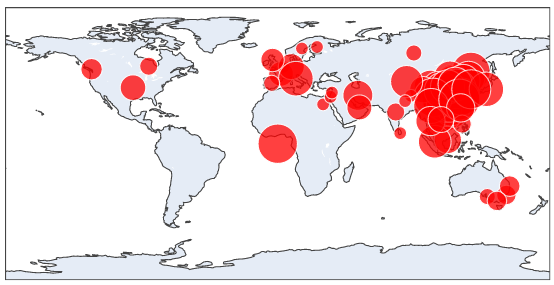
\includegraphics[width=0.9\linewidth]{../covid_spread_20200223.png}
      \caption{2020.02.23}
    \end{subfigure}
  \end{figure}

\end{frame}

\begin{frame}{Motivation (2/2)}

  \begin{figure}[!b]
    \centering
    \begin{subfigure}[b]{\linewidth}
      \centering
      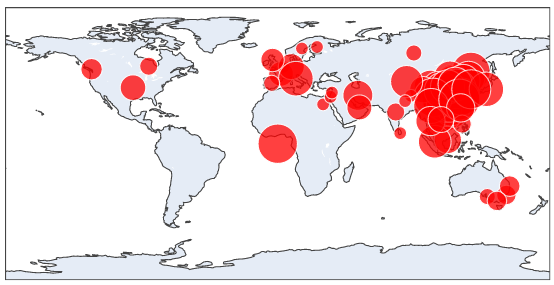
\includegraphics[width=0.5\linewidth]{../covid_spread_20200223.png}
      \caption{2020.02.23}
    \end{subfigure}
    \begin{subfigure}[b]{\linewidth}
      \centering
      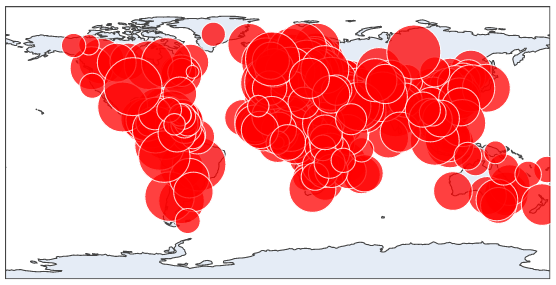
\includegraphics[width=0.5\linewidth]{../covid_spread_20200511.png}
      \caption{2020.05.11 [TODO: Current picture]}
    \end{subfigure}\\
  \end{figure}

\end{frame}

\begin{frame}{Proportional Symbol Maps}

  \begin{figure}[!b]
    \centering
      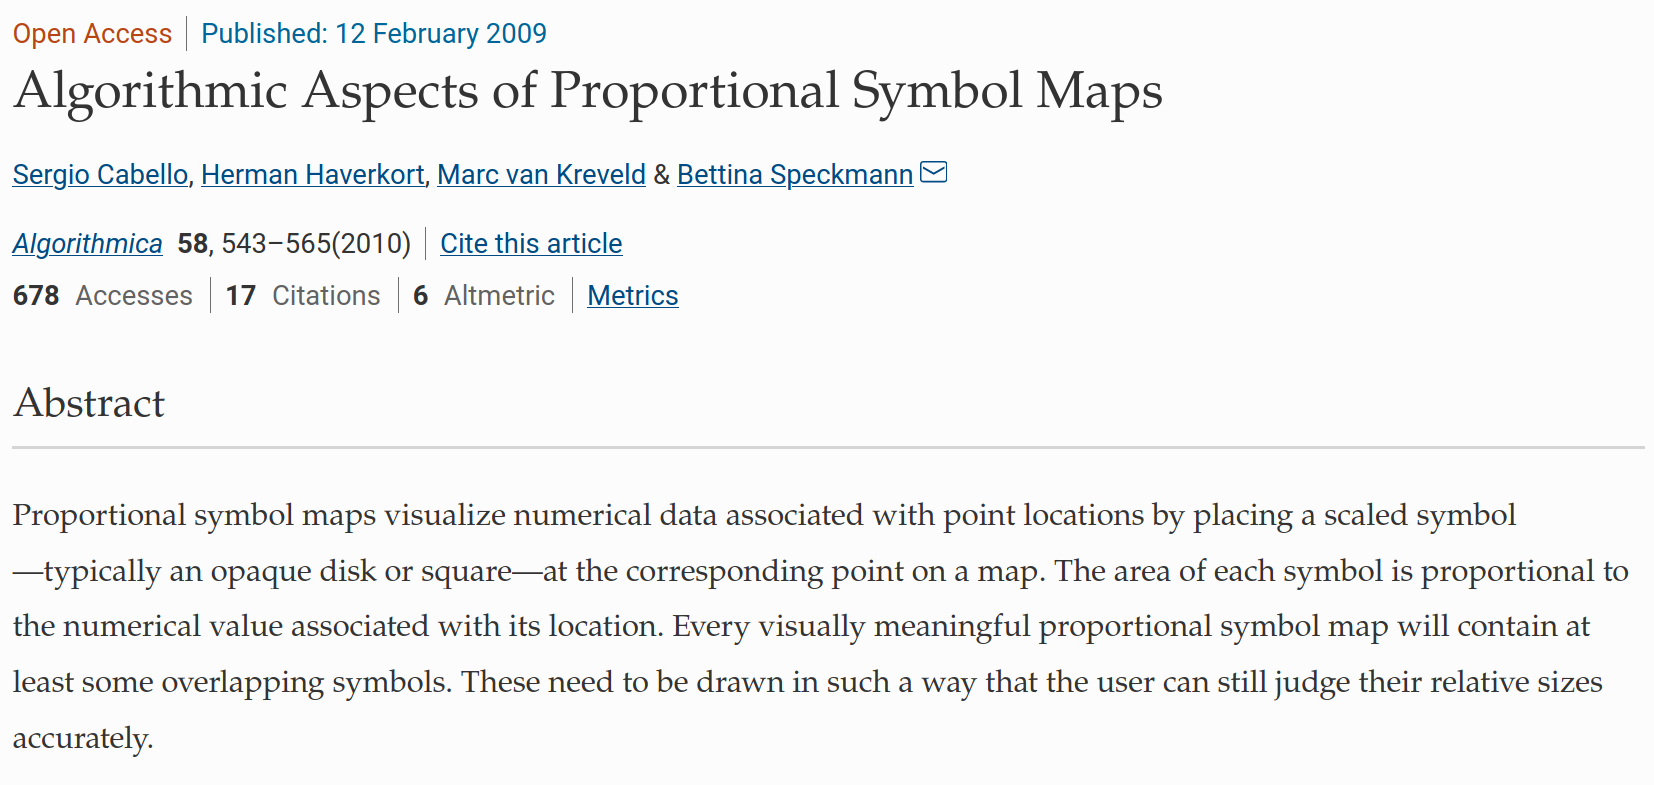
\includegraphics[width=0.9\linewidth]{assets/cabello_haverkort_image.png}
      \caption{Algorithmic Aspects of Proportional Symbol Maps}
  \end{figure}

\end{frame}

\begin{frame}{Physically realizable drawings}
  \begin{figure}[!b]
    \centering
      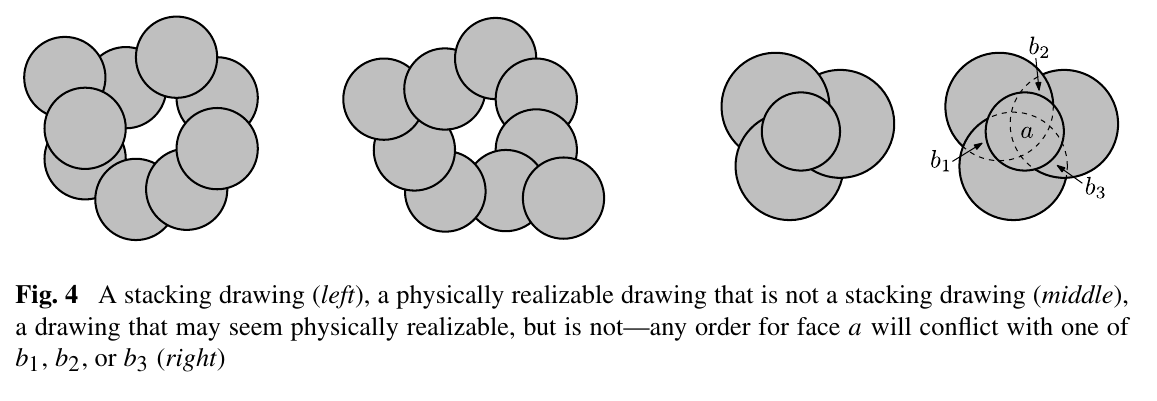
\includegraphics[width=0.9\linewidth]{assets/cabello_drawings.png}
      \caption{Physically realizable vs. stacking drawings vs. impossible}
  \end{figure}
\end{frame}

\begin{frame}{Utility functions}
\begin{align*}
  \lambda_{min} (D) & = \min_{i \in [n]}|U_i^{vis}| \\
  \\
  \lambda_{sum} (D) & = \sum_{i=1}^n|U_i^{vis}|
\end{align*}

\end{frame}

\begin{frame}{Why this lab?}

$$
\phi: \{1,...,n\} \mapsto D
$$

\end{frame}

\begin{frame}{Maps and Glyphs}
  \begin{figure}[!b]
    \centering
    \begin{subfigure}[b]{0.45\linewidth}
      \centering
      
\includegraphics[width=0.5\linewidth]{assets/symbol_nested_circles}
      \caption{Coffee.}
    \end{subfigure}
    \begin{subfigure}[b]{0.45\linewidth}
      \centering
      
\includegraphics[width=0.5\linewidth]{assets/symbol_nested_elastic_circles}
      \caption{More coffee.}
    \end{subfigure}\\
    \begin{subfigure}[b]{0.45\linewidth}
      \centering
      
\includegraphics[width=0.5\linewidth]{assets/symbol_pie}
      \caption{Tasty coffee.}
    \end{subfigure}
    \begin{subfigure}[b]{0.45\linewidth}
      \centering
      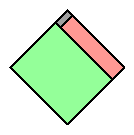
\includegraphics[width=0.5\linewidth]{assets/symbol_square}
      \caption{Too much coffee.}
    \end{subfigure}
  \end{figure}

\end{frame}

\section{Algorithms}

\begin{frame}{Visibility of general glyphs}
    \begin{itemize}
        \item assign local utility to each glyph
        \item define global utility as minimum (or sum) over all local utilities
        \item we will focus on minimum approaches
        \item examples
        \begin{enumerate}
            \item visibility (yes/no)
            \item visible area
            \item visible boundary length absolute or relative
            \item visibility of special points
        \end{enumerate}
    \end{itemize}
\end{frame}

\begin{frame}{Greedy Stackings}
    \textbf{Theorem:} Given as finite set $D$ of $n$ glyphs, a local utility function $\Gamma(d, S) \in \mathbb{R}_{>0}$ for $d\in D$ and $S\subseteq D$, which is anti-monotonous in $S$ and a global utility function $\lambda$ as the minimum of the local utilities, then the GreedyStacking algorithm computes an optimal stacking order.
    
    \pause
    
    \textbf{GreedyStacking(D)}\\
    if($D\neq \emptyset$) \{\\ 
        \tab$x=argmin_{d\in D} \Gamma(d, D\setminus d)$\\
        \tab$yield\ x$\\
        \tab$\textrm{\textbf{GreedyStacking}}(D\setminus x)$\\
    \}
\end{frame}

\begin{frame}{GreedyStacking}
    Give proof.
\end{frame}

\begin{frame}{Centered Nested circles}
  \pgfputat{\pgfxy(11.5, 0)}{\pgfbox[right,base]{
      
\includegraphics[width=1.2cm,height=1.2cm,keepaspectratio]{assets/symbol_nested_circles.pdf}
  }}
  \begin{itemize}
      \item natural generalization and seen in action
  \end{itemize}
  \begin{figure}[h]
    \centering
      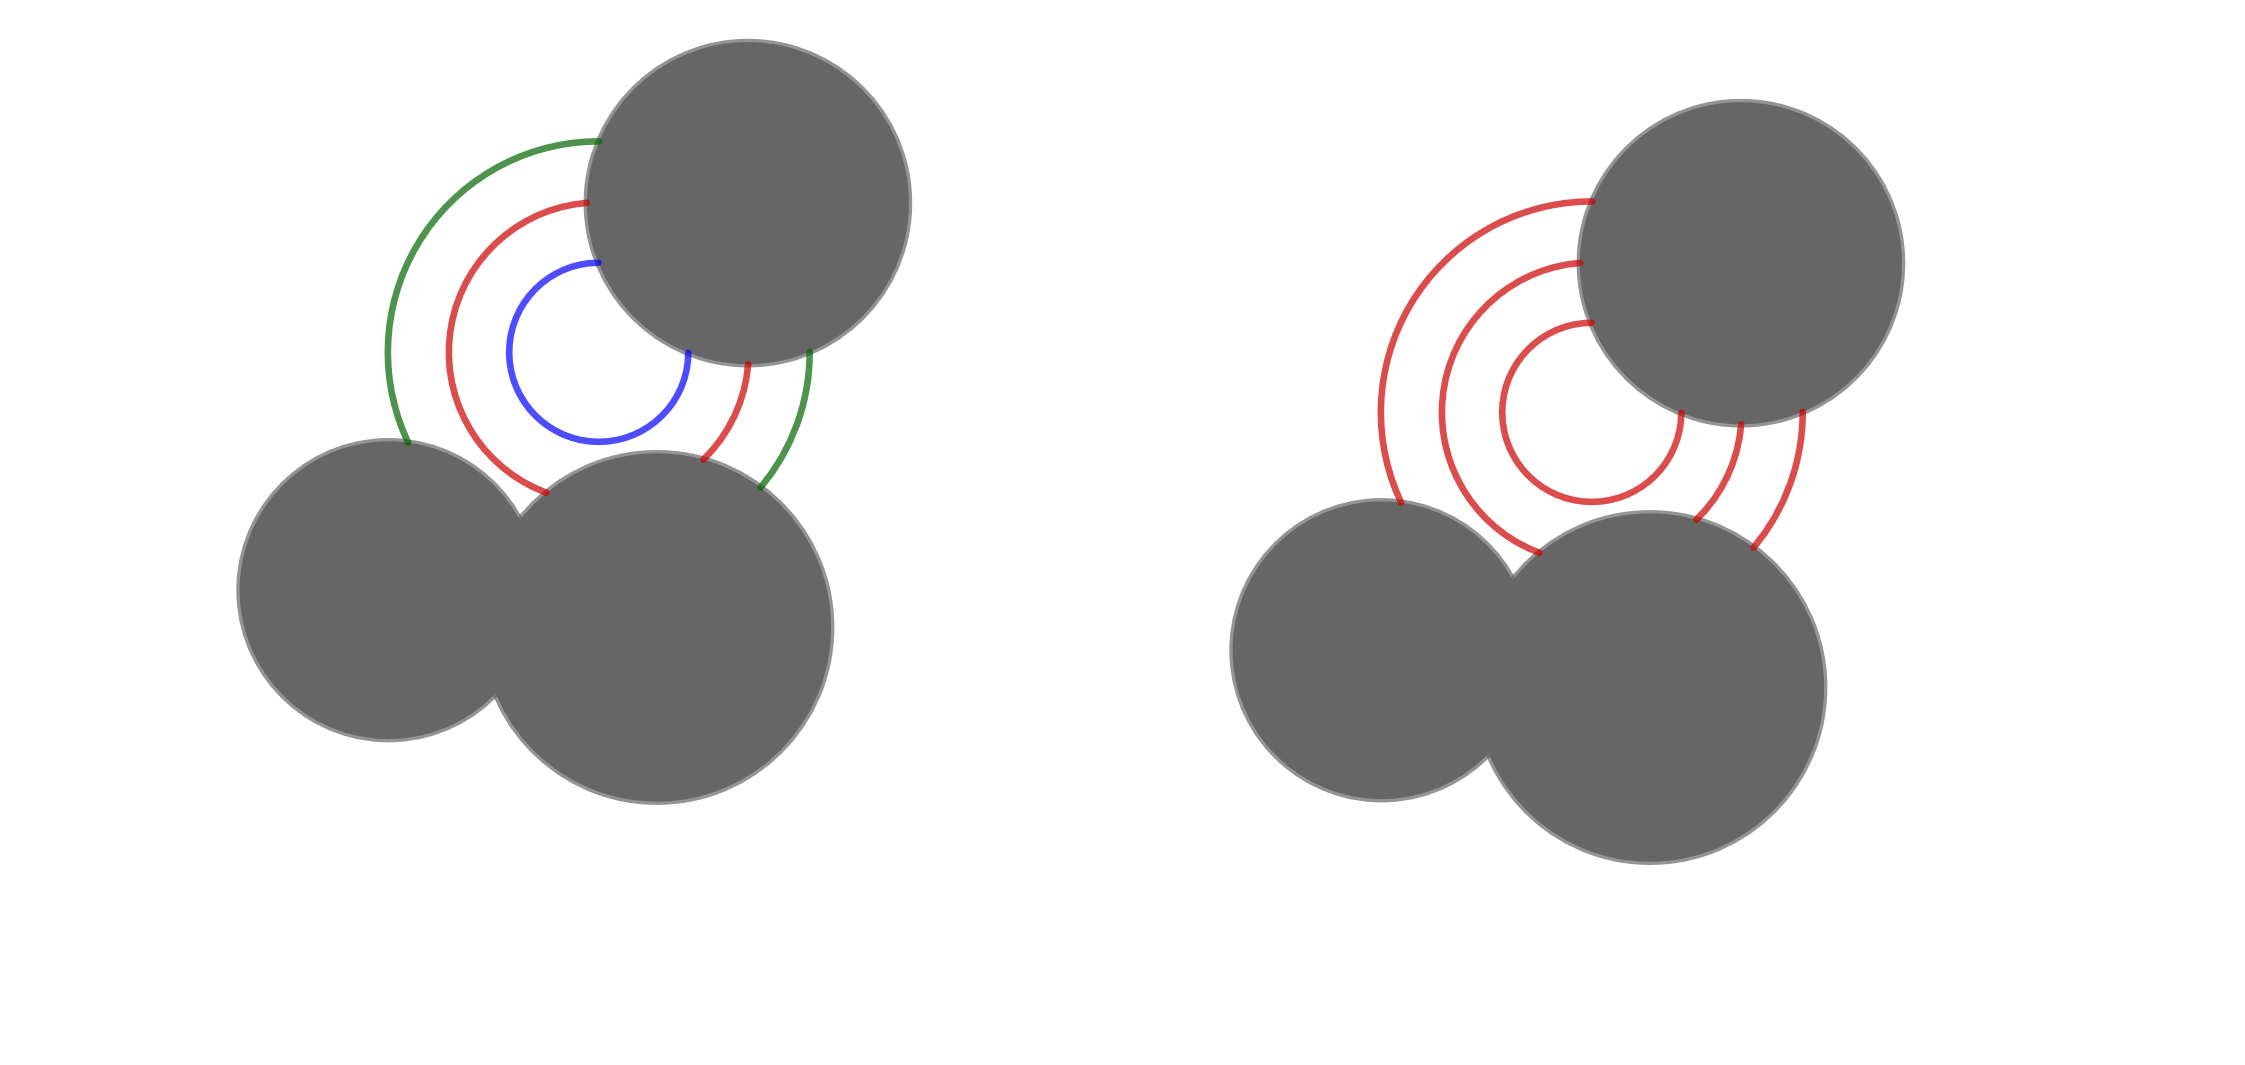
\includegraphics[width=0.9\linewidth]{slides/assets/nested_utility.png}
      \caption{Minimum attained at red circle}
  \end{figure}
  \begin{itemize}
      \item optimization is NP-hard for physically realizable
      \item greedy runs in $O(n^3\cdot k^2)$
  \end{itemize}
\end{frame}

\begin{frame}{Freely Nested circles}
  \pgfputat{\pgfxy(11.5, 1.8)}{\pgfbox[right,base]{
      
\includegraphics[width=1.2cm,height=1.2cm,keepaspectratio]{assets/symbol_nested_elastic_circles.pdf}
  }}
  \begin{itemize}
      \item allow to move disks inside
      \item same utility as above
      \item increased freedom comes with increased complexity
  \end{itemize}
  Freely nested disks are to complex to go over all possible placements $\implies$ simplify to Hawaiian Earring setup.
\end{frame}

\begin{frame}{Freely Nested circles}
  \pgfputat{\pgfxy(11.5, 0)}{\pgfbox[right,base]{
      
\includegraphics[width=1.2cm,height=1.2cm,keepaspectratio]{assets/symbol_nested_elastic_circles.pdf}
  }}
  
  \begin{itemize}
      \item all disks will be visible
      \item the greedy algorithm does NOT imply optimality
      \item verify into experiments
      \item greedy with longest continuous visible segment
  \end{itemize}
  
  \begin{figure}[h]
    \centering
      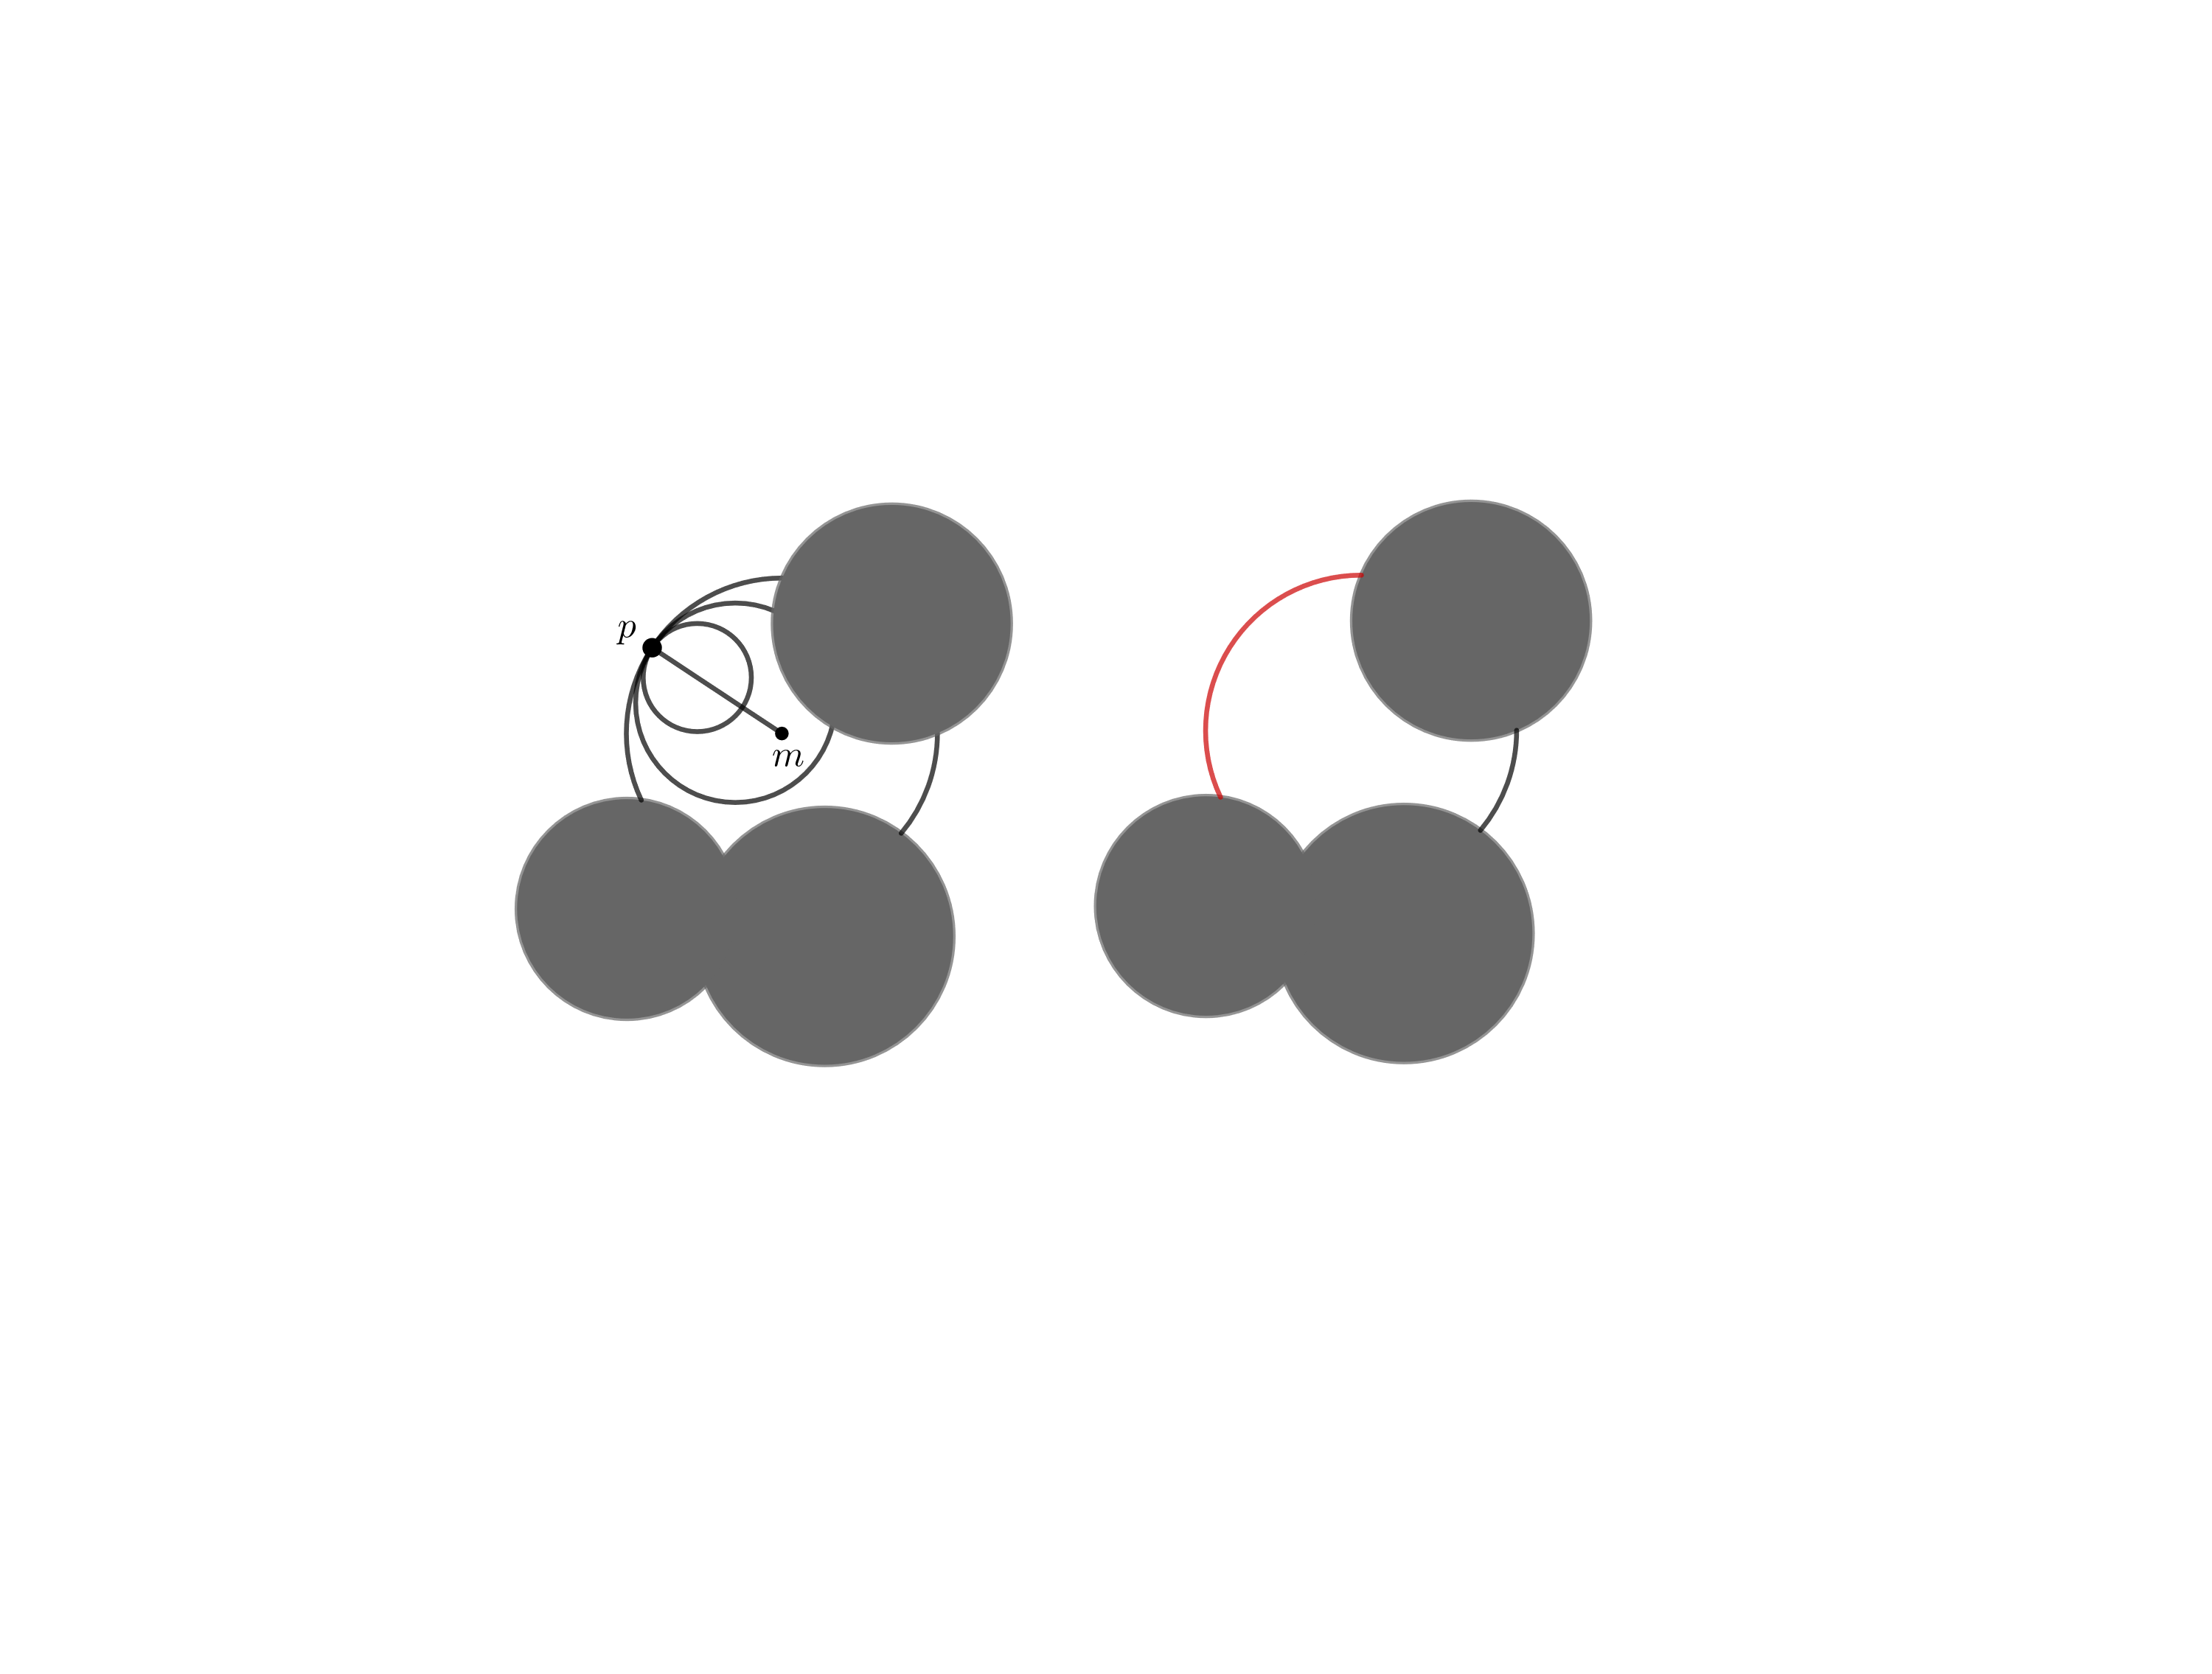
\includegraphics[width=0.9\linewidth]{slides/assets/hawaiian_utility.png}
  \end{figure}
  
\end{frame}

\begin{frame}{Pies}
  \pgfputat{\pgfxy(11.5, 3.5)}{\pgfbox[right,base]{
      
\includegraphics[width=1.2cm,height=1.2cm,keepaspectratio]{assets/symbol_pie.pdf}
  }}
\end{frame}

\begin{frame}{Squares}
  \pgfputat{\pgfxy(11.5, 3.5)}{\pgfbox[right,base]{
      
\includegraphics[width=1.2cm,height=1.2cm,keepaspectratio]{assets/symbol_square.pdf}
  }}
\end{frame}

\section{Experimental results}

\begin{frame}{Experimental Setup}
  \begin{itemize}
    \item We use the John Hopkins University Covid-19 data
    \item recovered are coloured green, deceased are coloured black and		the infected are coloured red
    \item logarithmic scaling dependent on two parameters:
      \begin{align*}
	r=M* \log \left( \frac{c_i S}{c_{max}} +1 \right)
      \end{align*}
      $M$ is the maximum size of a glyph, $S$ is a scaling factor and $c_{max}$ is			the maximum number of cases
  \end{itemize}
\end{frame}



\begin{frame}

  \begin{figure}[!t]
    \centering
    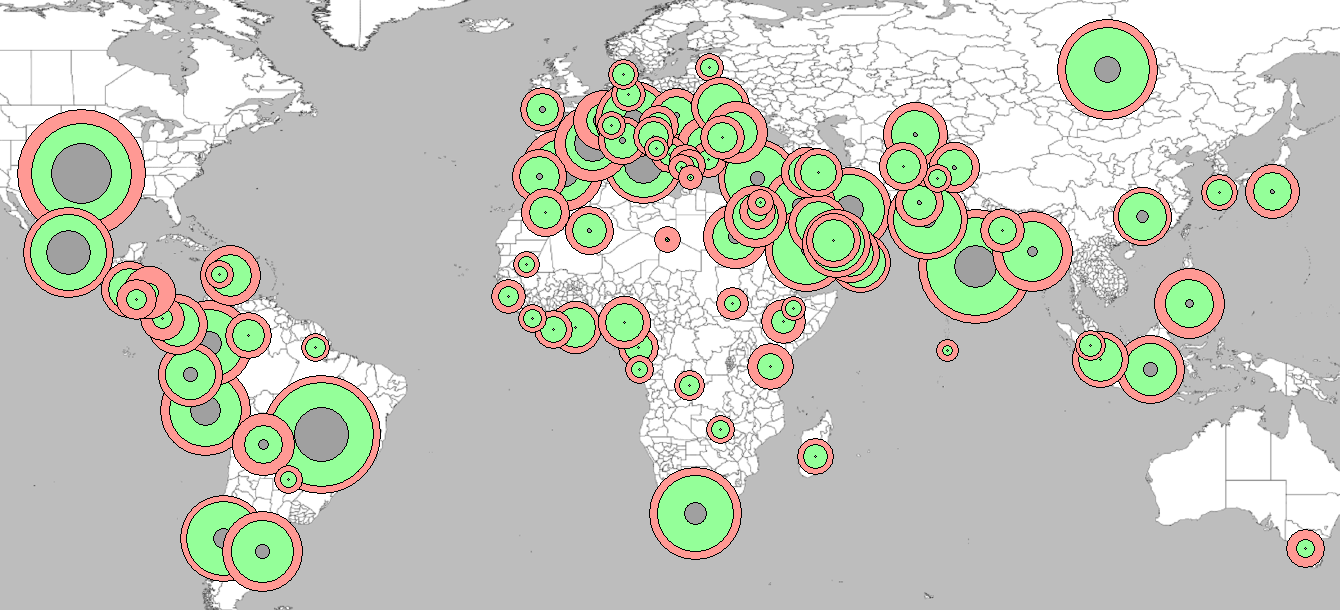
\includegraphics[height=4.5cm]{assets/MinMinAbsEval.png}
  \end{figure}
%
  \begin{table}
    \resizebox{9cm}{!}{%
      \begin{tabular}{| l || p{1.3cm} | p{1.7cm} | p{1.7cm} | p{1.5cm} | p{1.5cm} | p{1.5cm} |}
	\hline
	algorithm            & covered & minVis (rel) & minVis (abs) & min one glyph & average rel vis & absolute perc \\
	\hline
	random               &  {44}      & 0.011 (0)    & 0.995 (0)    & 0             & 0.658           & 0.677         \\

	LeftToRight          &  {42}      & 0.053 (0)    & 2.189 (0)    & 0             & 0.641           & 0.678         \\

	RightToLeft          &{  43}      & 0.053 (0)    & 0.995 (0)    & 0             & 0.656           & 0.693         \\
	\hline
	Painter              & {  16 }     & 0.064 (0)    & 6.283 (0)    & 34.991        & 0.761           & 0.718
	\\

	MinMinStacking (abs) & {  16 }     & 0.075 (0)    & 2.189 (0)    & 44.467        & 0.757           & 0.724         \\

	\hline
	MinMinStacking (rel) & { 18 }     & 0.11 (0)    & 2.189 (0)    & 37.327        & 0.748           & 0.725         \\

	MinSumStacking (abs) & \red{ 18}      & 0.111 (0)    & 3.974 (0)    & \red{44.467}        & 0.75            & 0.721         \\

	MinSumStacking (rel) &{  18 }     & 0.111 (0)    & 2.189 (0)    & 37.327        & 0.744           & 0.723         \\

	\hline
    \end{tabular}}
    \caption{{\footnotesize Date: 02.08.2020, $n_{records}:$ 78, parameters: $M=50$, $S=500$ and $\text{minimum number of cases}=5000$}}
  \end{table}
\end{frame}

\begin{frame}
  \begin{figure}[!t]
    \centering
    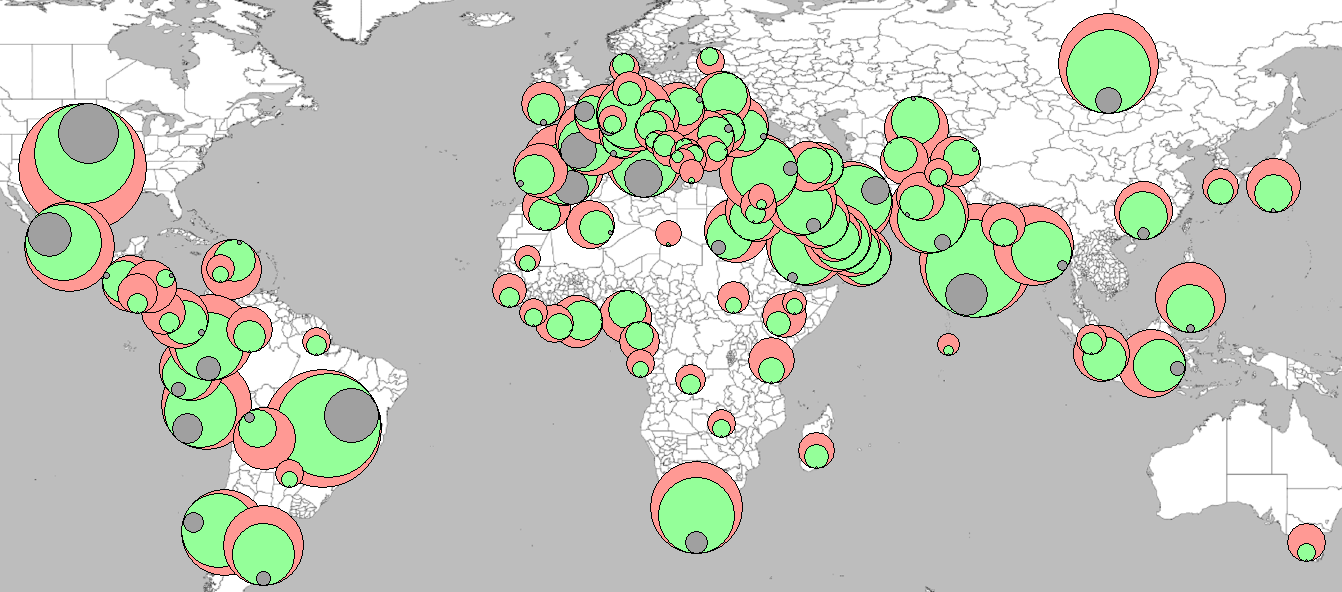
\includegraphics[height=5cm]{assets/hawaiianEval.png}
  \end{figure}
  \begin{table}[!h]
    \begin{center}
      \resizebox{9cm}{!}{%
	\begin{tabular}{| l || p{1.3cm} | p{1.7cm} | p{1.7cm} | p{1.5cm} | p{1.5cm} | p{1.5cm} |}
	  \hline
	  algorithm    & covered & minVis (rel) & minVis (abs) & min one Glyph & average rel vis & absolute perc \\
	  \hline
	  random       & 21      & 0.0001 (0)    & 0.589 (0)    & 0             & 0.765           & 0.714         \\

	  LeftToRight  & 12      & 0.15 (0)    & 2.743 (0)    & 0             & 0.775           & 0.725         \\

	  RightToLeft  & 13      & 0.106 (0)    & 2.89 (0)     & 0             & 0.783           & 0.735         \\
	  \hline
	  Painter      & \red 0       & \red{0.093}        & 6.283        & 47.758        & 0.857           & 0.759         \\

	  our Stacking & \red 0       & \red{ 0.373 }       & 6.283        & 75.034        & 0.859           & 0.77          \\

	  \hline
      \end{tabular}}
    \end{center}
    \caption{date: 02.08.2020  , $M=50$, $S=500$ and $\text{MnC}=5000$  }
  \end{table}
\end{frame}


\begin{frame}
  \begin{table}
    \resizebox{9cm}{!}{%
      \begin{tabular}{| l || p{1.3cm} | p{1.7cm} | p{1.7cm} | p{1.5cm} | p{1.5cm} | p{1.5cm} |}
	\hline
	algorithm            & covered & minVis (rel) & minVis (abs) & min one glyph & average rel vis & absolute perc \\
	\hline
	random               & 44      & 0.011 (0)    & 0.995 (0)    & 0             & 0.658           & 0.677         \\

	LeftToRight          & 42      & 0.053 (0)    & 2.189 (0)    & 0             & 0.641           & 0.678         \\

	RightToLeft          & 43      & 0.053 (0)    & 0.995 (0)    & 0             & 0.656           & 0.693         \\
	\hline
	Painter              &  \red{16}        & 0.064 (\red 0)    & 6.283 (0)    & 34.991        & \red {0.761}           & \red {0.718}         \\

	MinMinStacking (abs) & \red{16}      & 0.075 (\red 0)    & 2.189 (0)    & 44.467        & \red {0.757}           & \red {0.724}         \\
	\hline
	MinMinStacking (rel) & 18      & 0.11 (0)    & 2.189 (0)    & 37.327        & 0.748           & 0.725         \\

	MinSumStacking (abs) & 18      & 0.111 (0)    & 3.974 (0)    & 44.467        & 0.75            & 0.721         \\

	MinSumStacking (rel) & 18      & 0.111 (0)    & 2.189 (0)    & 37.327        & 0.744           & 0.723         \\

	\hline
    \end{tabular}}
    \caption{centered disks  }
  \end{table}
  \begin{table}[!h]
    \begin{table}[!h]
      \begin{center}
	\resizebox{9cm}{!}{%
	  \begin{tabular}{| l || p{1.3cm} | p{1.7cm} | p{1.7cm} | p{1.5cm} | p{1.5cm} | p{1.5cm} |}
	    \hline
	    algorithm    & covered & minVis (rel) & minVis (abs) & min one Glyph & average rel vis & absolute perc \\
	    \hline
	    random       & 21      & 0.0001(0)    & 0.589 (0)    & 0             & 0.765           & 0.714         \\

	    LeftToRight  & 12      & 0.15 (0)    & 2.743 (0)    & 0             & 0.775           & 0.725         \\

	    RightToLeft  & 13      & 0.106 (0)    & 2.89 (0)     & 0             & 0.783           & 0.735         \\
	    \hline
	    Painter      &\red 0       & 0.093        & 6.283        & 47.758        & \red{ 0.857  }         & \red{ 0.759  }       \\

	    our Stacking &\red 0       & \red{0.373}        & 6.283        & 75.034        & \red{ 0.859 }     &     \red{ 0.77 }        \\

	    \hline
	\end{tabular}}
      \end{center}
      \caption{
      date: 02.08.2020  , $M=50$, $S=500$ and $\text{MnC}=5000$ }
    \end{table}
  \end{table}
\end{frame}


\begin{frame}
  \begin{figure}[!t]
    \centering
    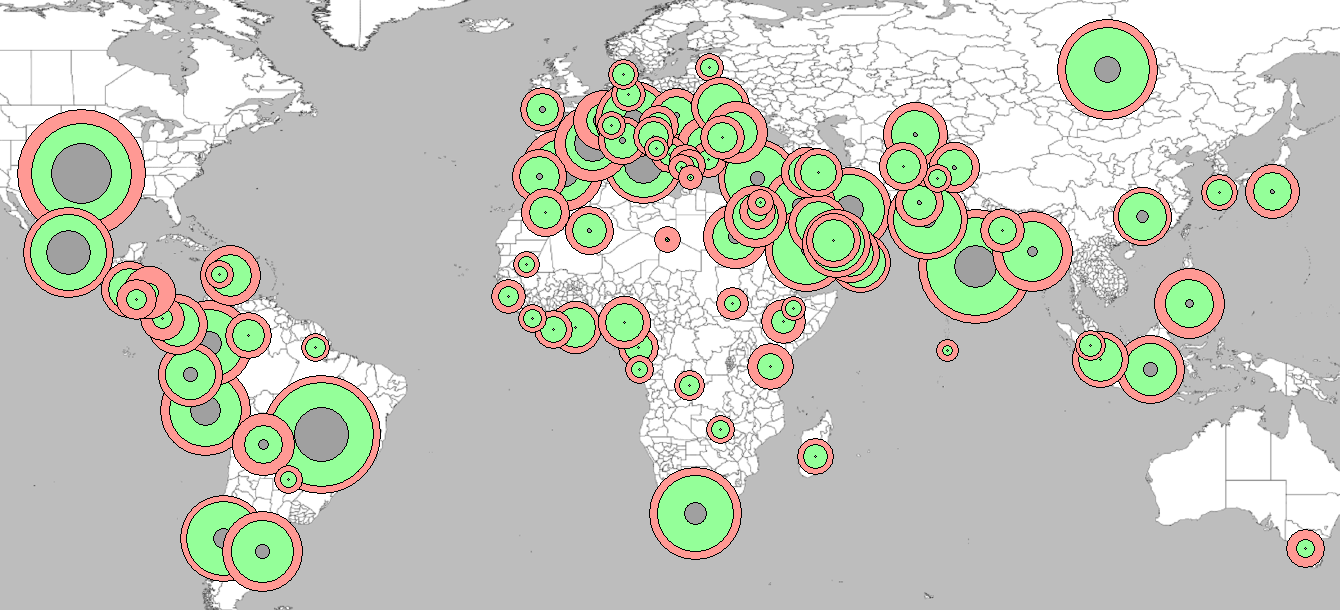
\includegraphics[height=4cm]{assets/MinMinAbsEval.png}
  \end{figure}
  \begin{figure}[!t]
    \centering
    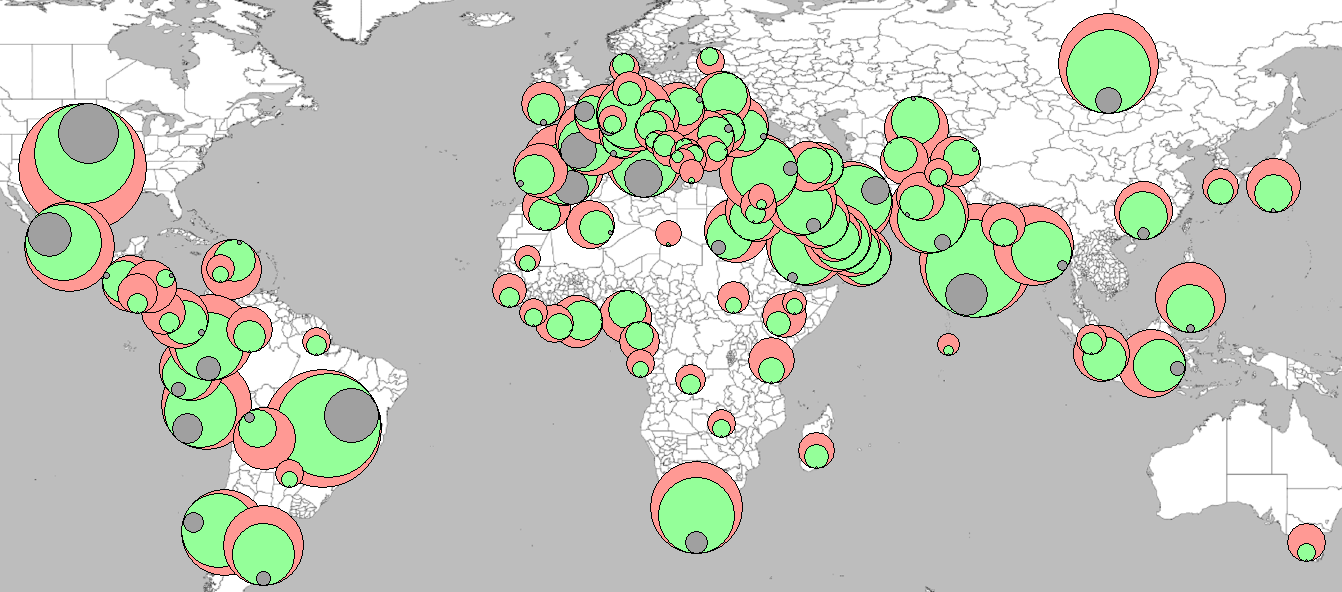
\includegraphics[height=4cm]{assets/hawaiianEval.png}
  \end{figure}
\end{frame}


\begin{frame}
  \begin{figure}[!b]
    \centering
    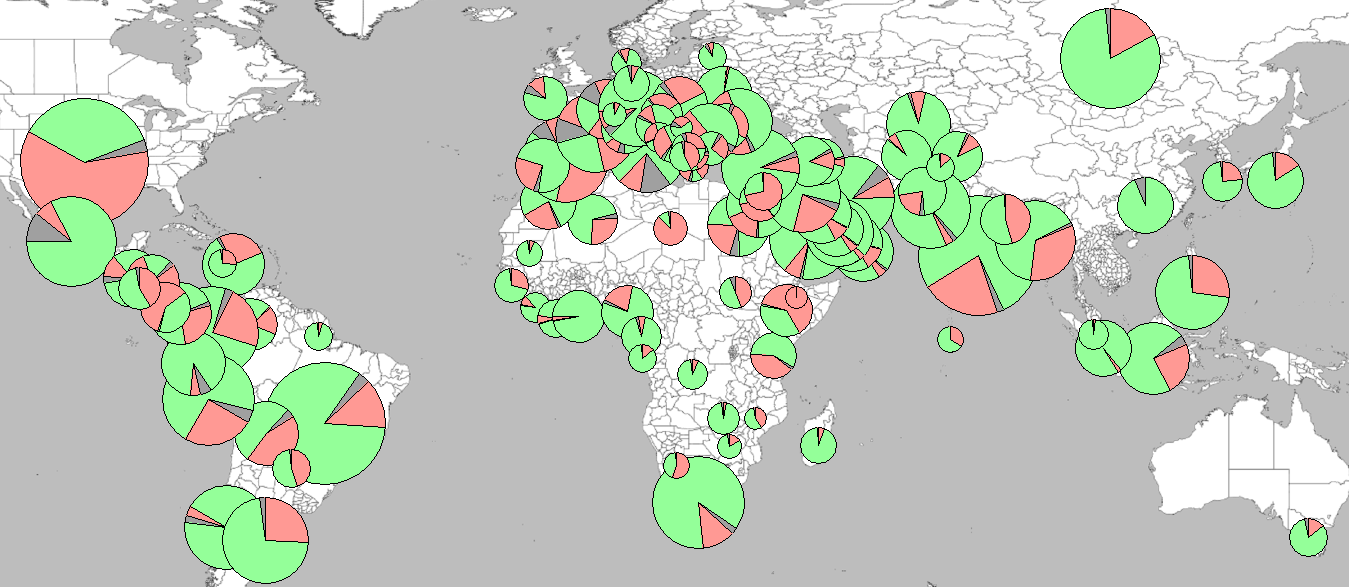
\includegraphics[height=5cm]{assets/pieChartsEval.png}
  \end{figure}
  \begin{table}[h]
    \begin{center}\resizebox{7cm}{!}{
	\begin{tabular}{| l || l | l | l | l |}
	  \hline
	  algorithm          & covered & minDist (rel)   & minDistAvg (rel) & minDistAvg (abs) \\
	  \hline
	  Painter+random     & \red{80}    & 0.0 (0) & 1.01     & 24.266    \\

	  random+heuristic   & 29      & 0.0 (0)   & 1.587     & 42.946     \\

	  RightToLeft        & 18      & 0.017 (0) & 1.621      & 43.407     \\
	  \hline
	  Painter+ heuristic & \red{5 }      & 0.022 (0) & 1.706      & 41.719   \\

	  our Stacking       & \red{0}     & 0.271     & 1.765      & 44.452      \\

	  \hline
      \end{tabular}}
    \end{center}
    \caption{ date: 22.08.2020, $M=50$, $S=500$ and $\text{MnC}=5000$  }
  \end{table}
\end{frame}


\begin{frame}
  \begin{figure}[b]
    \centering
    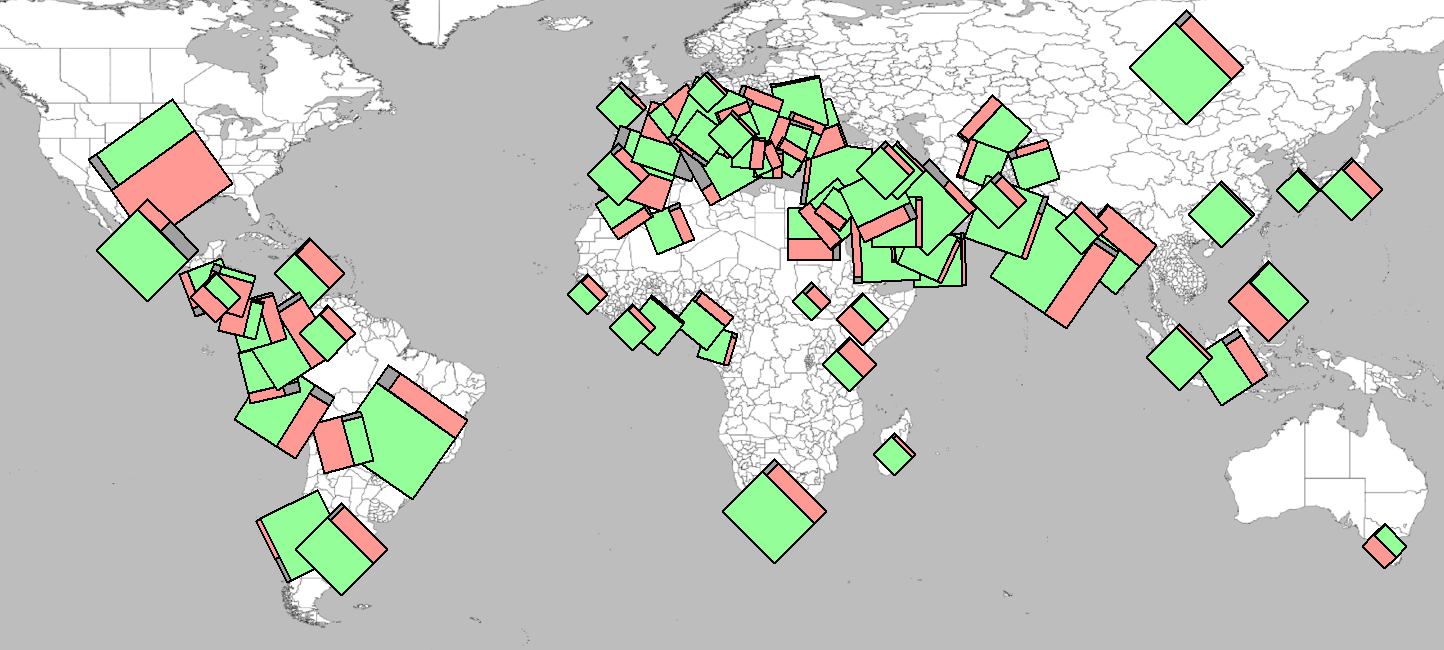
\includegraphics[height=5cm]{assets/squaresEval.png}
  \end{figure}
  \begin{table}[h]
    \begin{center}
      \resizebox{7cm}{!}{
	\begin{tabular}{| l || l | l | }
	  \hline
	  algorithm                           & covered & minDist \\  %& minDistAvg \\
	  \hline

	  random Stacking+random rotations    & 87      & 0.235 (0)\\ %& 35.846     \\

	  Painter+random rotations            & 41     & 0.58 (0)\\ %& 34.406     \\

	  random Stacking+heuristic rotations & 56    & 0.027 (0)\\ %& 34.776     \\
	  \hline
	  Painter+heuristic                   & \red{19}      & 0.052 (0)\\ %& 32.061     \\

	  our Stacking                        & \red{ 13}       & 0.052 (0)\\ %& 25.232     \\

	  \hline
      \end{tabular}}
    \end{center}
    \caption{
    date: 22.08.2020  , $M=50$, $S=500$ and $\text{MnC}=5000$  }
  \end{table}
\end{frame}


\begin{frame}
  \begin{figure}[!b]
    \centering
    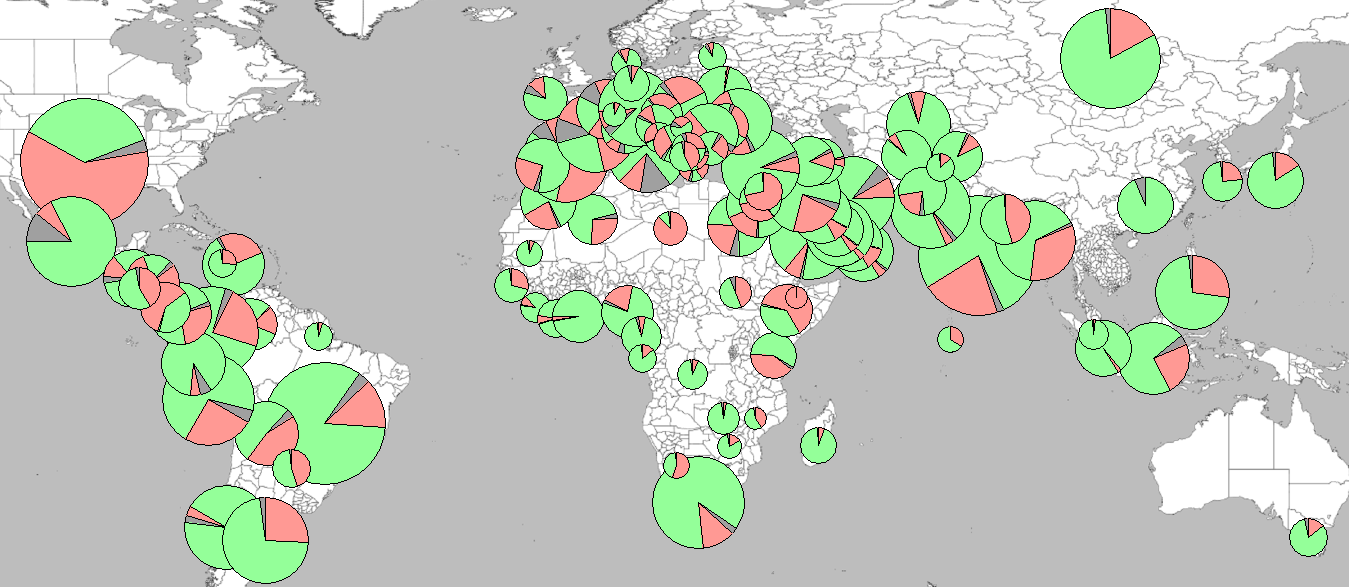
\includegraphics[height=4.2cm]{assets/pieChartsEval.png}
  \end{figure}

  \begin{figure}[b]
    \centering
    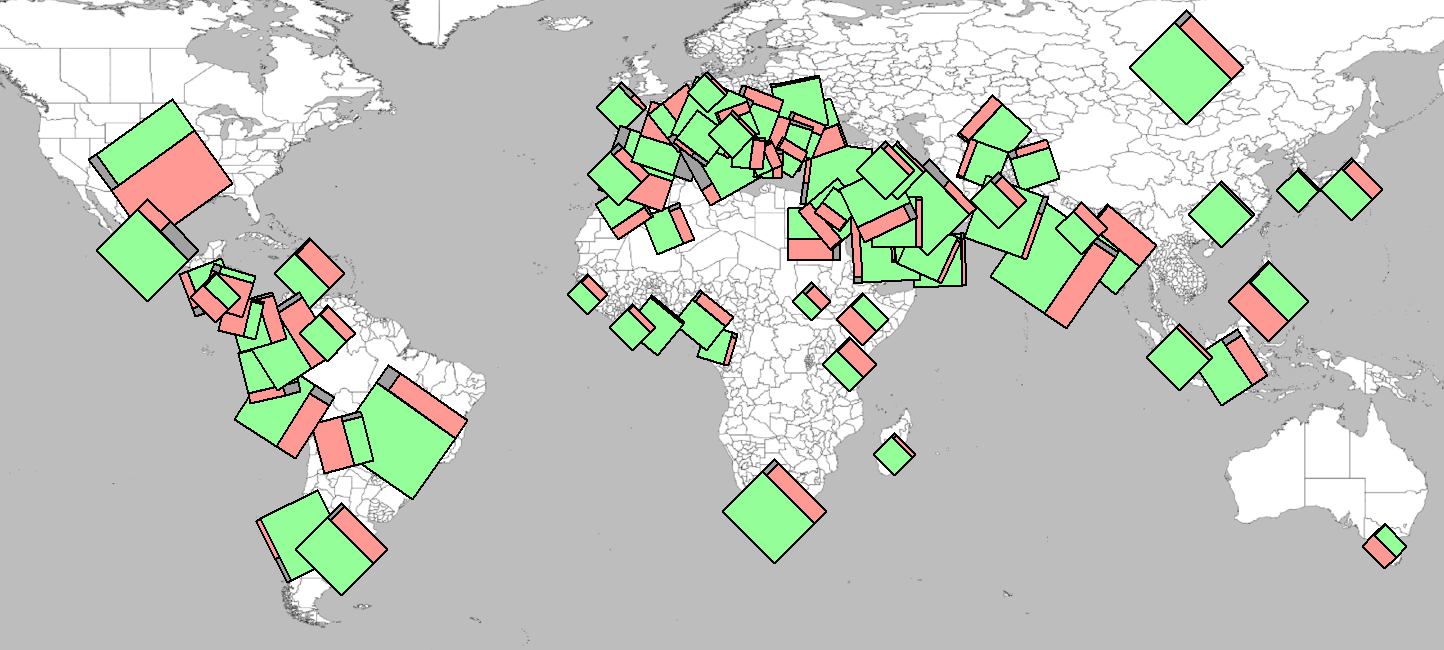
\includegraphics[height=4.2cm]{assets/squaresEval.png}
  \end{figure}
\end{frame}



\section{Exploration in App}

\begin{frame}{Exploration of the data}
  [Switch to app and play!]
\end{frame}

\section{Conclusion and Outlook}

\begin{frame}{Summary}

  \begin{itemize}
    \item Four glyphs were shown, with two new approaches.
    \item NP-hardness of new approaches was outlined.
    \item Heuristics and greedy approach usually are good choices.
    \item Square/pie approach can be interpreted as discrete version of the relative visibility.
    \item All of this was verified on the most recent COVID-19 data,
    \item and experimentally demonstrated.
  \end{itemize}
\end{frame}

\end{document}

